\documentclass[tikz]{standalone}

\definecolor{n0}{HTML}{785EF0}
\definecolor{End}{HTML}{DC267F}
\definecolor{Corner}{HTML}{FFB000}
\definecolor{NewHex}{HTML}{648FFF}
\definecolor{Reversal}{HTML}{FE6100}

\begin{document}
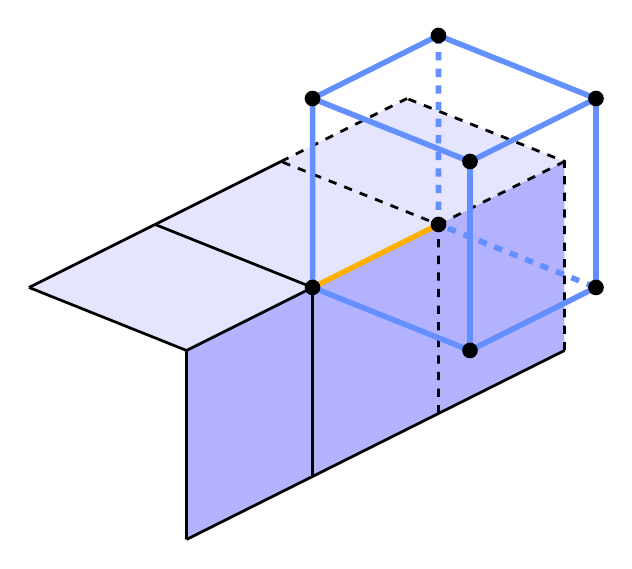
\begin{tikzpicture}[scale=4, x={(0.5cm,-0.2cm)}, y={(0.4cm,0.2cm)}, z={(0.0cm,0.6cm)}]

  %%%%%%%%%% Points pour travailler %%%%%%%%%%
 \coordinate (0) at (0,0,0);
 \coordinate (1) at (0,1,0);
 \coordinate (2) at (0,2,0);
 \coordinate (3) at (0,3,0);
 \coordinate (4) at (0,0,1);
 \coordinate (5) at (0,1,1);
 \coordinate (6) at (0,2,1);
 \coordinate (7) at (0,3,1);
 \coordinate (8) at (1,1,1);
 \coordinate (9) at (1,2,1);
 \coordinate (10) at (-1,0,1);
 \coordinate (11) at (-1,1,1);
 \coordinate (12) at (-1,2,1);
 \coordinate (13) at (-1,3,1);
 \coordinate (14) at (0,1,2);
 \coordinate (15) at (0,2,2);
 \coordinate (16) at (1,1,2);
 \coordinate (17) at (1,2,2);

 %%%%%%%%%% Layer blue color %%%%%%%%%%
 \fill [color=blue!30!white] (4) -- (7) -- (3) -- (0) -- cycle ;
 \fill [color=blue!10!white] (4) -- (7) -- (13) -- (10) -- cycle ;
 
 % Layer 1
 \draw [line width=1] (0) -- (3) ;
 \draw [line width=1] (4) -- (5) ;
 \draw [dashed, line width=1] (6) -- (7) ;
 \draw [line width=1] (10) -- (12) ;
 \draw [dashed, line width=1] (12) -- (13) ;
 
 \draw [line width=1] (0) -- (4) -- (10) ;
 \draw [line width=1] (1) -- (5) -- (11) ;
 \draw [dashed, line width=1] (2) -- (6) -- (12) ;
 \draw [dashed, line width=1] (3) -- (7) -- (13) ;

 %%%%%%%%%%% Feature edge %%%%%%%%%%%
 \draw [line width=2, color=Corner] (5) -- (6) node[pos=0.6, color=black, opacity=0.7, below] {} ;
 
 %%%%%%%%%%% The HEXA created %%%%%%%%%%%
 \draw [line width=2, color=NewHex] (5) -- (8) -- (16) -- (14) -- (5) ;
 \draw [line width=2, color=NewHex] (16) -- (17) -- (9) -- (8) ;
 \draw [line width=2, color=NewHex] (14) -- (15) -- (17) -- (9) ;

 \draw [dashed, line width=2, color=NewHex] (15) -- (6) -- (9) ;

%%%%%%%%%%% HEXA NODES %%%%%%%%%%%
 \draw (5) node[circle, fill=black, inner sep = 2 pt] {};
 \draw (6) node[circle, fill=black, inner sep = 2 pt] {};
 \draw (8) node[circle, fill=black, inner sep = 2 pt] {};
 \draw (9) node[circle, fill=black, inner sep = 2 pt] {};
 \draw (14) node[circle, fill=black, inner sep = 2 pt] {};
 \draw (15) node[circle, fill=black, inner sep = 2 pt] {};
 \draw (16) node[circle, fill=black, inner sep = 2 pt] {};
 \draw (17) node[circle, fill=black, inner sep = 2 pt] {};
 
 %\draw (4) node[circle, fill=black, inner sep = 2 pt] {};

 %\foreach \i in {0,...,17}
 %{
 %  \draw (\i) node[circle, fill=black, inner sep = 2 pt] {};
 %}


\end{tikzpicture}
\end{document}